%!TEX root = ../talk.tex

\chapter{Comparison of IoT Business Model Frameworks}
\markboth{Comparison of IoT Business Model Frameworks}{}
\chaptauthors{Matthias Diez, Christian Ott, Silas Weber}

\Kurzfassung{
	With the emergence and spread of the `Internet of Things' (short IoT), businesses face a new challenge to stay productive and exploit the new technologies in a changing technological environment. Due to the inherent networked nature of IoT, businesses need to apply adapted business models in order to prevail in the IoT market. \\
	In this paper, we analyze how business model frameworks have changed due to the ongoing developments in the IoT industry compared to traditional industries. We do this by first giving an introduction into the `Internet of Things'. Then, we present traditional as well as specific IoT business models frameworks. The core of our seminar reports is the comparison of the discovered IoT business model frameworks by applying them to a fictional use case. We found that the reviewed IoT business model frameworks tend to shift their focus towards value creation and collaboration. Further, we found that the ecosystem framework is yet in its infancy and is difficult to apply to our use case. However, the three-dimensional collaborator framework, combining the ecosystem and traditional canvas view, worked well for our use case and proves to be a ready-to-use framework for IoT businesses today.
}


\newpage

\minitoc %Das Inhaltsverzeichnis

\newpage

\renewcommand{\labelitemii}{$\diamond$}
\renewcommand{\labelitemiii}{$\circ$}

\section{Introduction}
	Introduction of technology innovation always leads to innovation in business models. With the emergence of the `Internet of Things' (short IoT), business models become possible that were unthinkable in the past. Developing business models in an emergent technology field can be challenging. Business model frameworks can help innovators to come up with better economic solutions for their business idea. Therefore it is important that frameworks adapt to technical and economical changes in their respective business environment. 

	The goal of this paper is fourfold. First a common ground should be built, with definitions and characterizations of the `Internet of Things', business models and business model frameworks. Second, the basic business model framework concepts `Magic Triangle' and `Business Model Canvas' should be introduced. Third, it should be examined what changes were made to business model frameworks due to the development of IoT, and lastly, the currently available IoT business model frameworks should be presented and compared against each other.

	This seminar report is therefore structured as follows. In Section~\ref{sec:iot}, the term `Internet of Things' is introduced and its definition, growth, architecture and potential of IoT for business is evaluated. Section~\ref{sec:bmf} presents the concept of business models and business model frameworks. Along with the definitions, two major `classic' business model frameworks are described. Section~\ref{sec:bmf_available} shows available business model frameworks that are adapted for IoT. After that, those frameworks are compared using a fictitious company as an illustrative example in Section~\ref{sec:bmf_comparison}. In Section~\ref{sec:eval}, the findings of the previous sections are evaluated. Finally, a summary of the report as well as a conclusion about the current state of IoT business model frameworks are presented in Section~\ref{sec:summary}. 
 
\section{Internet of Things}
\label{sec:iot}
	The term `Internet of Things' has grown to be a major topic in academia and industry \cite{ju}. The phrasing was first used by Kevin Ashton during a presentation in 1998 \cite{westerlund}. From there, IoT has become a new paradigm postulating the ``interconnection of physical objects, by equipping them with sensors, actuators and a means to connect to the Internet'' \cite[p.~672]{dijkman}.

	Even though the term `Internet of Things' is currently used by everyone, there is no common consent about its definition. The International Telecommunication Union (ITU) defined IoT as ``a global infrastructure for the information Society, enabling advanced services by interconnecting (physical and virtual) things based on, existing and evolving, inter-operable information and communication technologies'' \cite[p.~1]{itu} in a recommendation published in 2012. Besides ITU's view of IoT, other definitions were proposed. Atzori et al. \cite{atzori} identified three visions of how IoT may be seen. As illustrated in Figure~\ref{fig:iot_visions}, one vision focuses on the `things' being connected over technologies like RFID, WLAN or NCF. The second, `Internet-oriented' view envisions anything being connected with anything. The third point of view is a `semantic-oriented' vision. Definitions found in literature predominantly focus on this vision. The `Semantic-oriented' vision present thoughts on problems generated through the extremely increased number of connected `things', e.g. the challenging issues related to the representation, storage, interconnection, search and organization of information from IoT. Due to the differences in these visions, the definitions of IoT established by organizations or entities vary strongly depending on their specific interests, approach taken on the subject as well as their backgrounds. The convergence of these three visions illustrated in Figure~\ref{fig:iot_visions} can be seen as the overall paradigm of IoT. This converged perspective is the one that this report takes on in the remaining sections. 

	\begin{figure}[ht]
	    \begin{center}
	    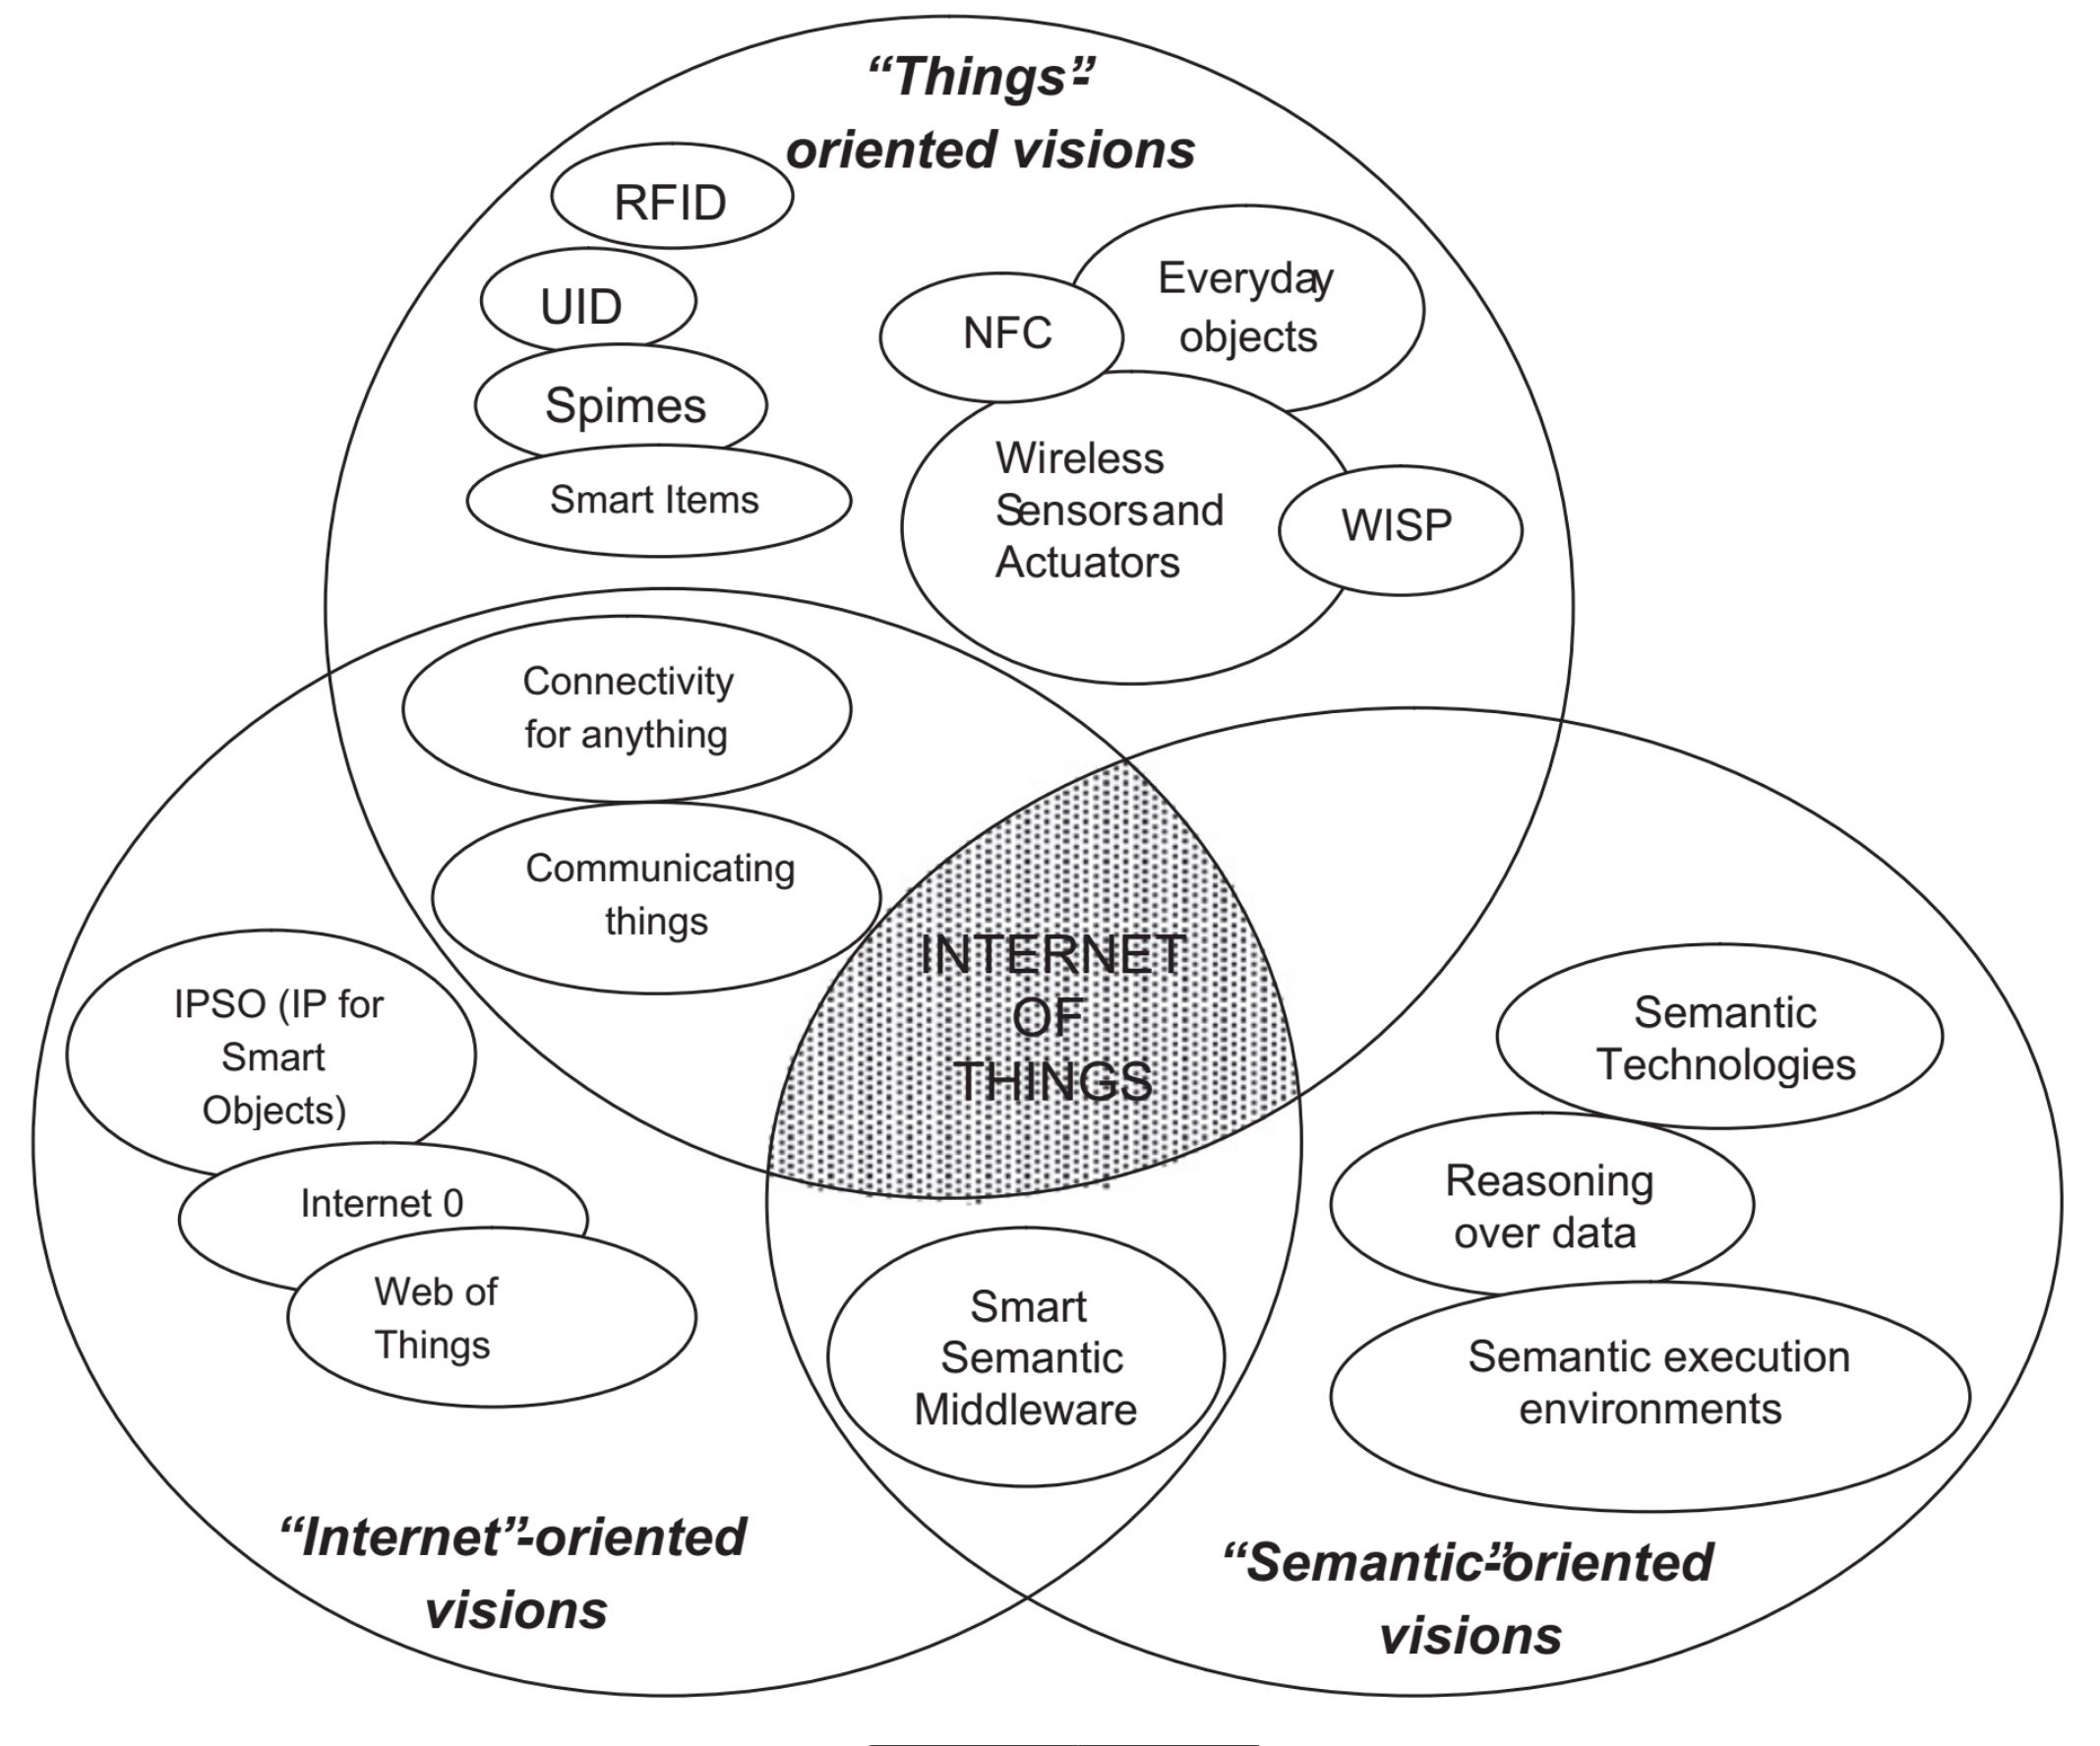
\includegraphics[scale=0.35]{Talk11/iot_visions.jpg}
	    \end{center}
	    \caption{`Internet of Things' paradigm as a result of the convergence of different visions(from Atzori et al. \cite{atzori})}
	    \label{fig:iot_visions}
    \end{figure}

	The number of worldwide connected `things' is rapidly growing. In 2016, Gartner predicted up to 6.4 billion connected devices which will rise up to 20.8 billion by 2020 \cite{gartner}. Consequently, organizations are more and more involved in IoT-related products, applications and services either in the development or as an investment \cite{ju}. Google spent \$3.2 billion to acquire Nest, a quickly growing smart thermostat company \cite{tilley_nest}. Samsung bought SmartTings, an open smart home platform \cite{tilley_smart}. Many IoT companies such as LiFX, a smart bulb company from San Francisco are emerging at the moment. LIFX came to through KickStarter \cite{kickstart}, a crowd-sourcing platform, and is today fully integrated with other smart home providers like the previously mentioned Nest and SmartThings. LIFX also works with Amazon Echo \cite{echo} or IFTTT \cite{ifttt}, both merge a diversity of services and provide a single access point. Telecommunication organizations invest in future technologies such as 5G which was discussed in Chapter 10 of this seminar report. Governments increasingly acknowledge the importance of IoT. The United States supported a Smart Cities Initiative with \$160 million \cite{miller}, and the Korean government planned investments of \$5 billion in various IoT projects until 2020 \cite{cho}. The investments driven by national institutions as well as aggressive investments by companies in IoT are expected to ``create new business opportunities and substantial social and economic benefits''\cite{ju}. 

	Even though there is no concrete definition what IoT is, there is some consent about the underlying architecture of IoT. A three-layered application stack can be found in various research literature. Albeit the layers may be named differently or subdivided into more layers, they are semantically comparable \cite{fleisch} \cite{ju}, \cite{wortmann}. In Figure~\ref{fig:wortmann_stack} the layered approach from Wortmann et al. is illustrated \cite{wortmann}. They presented a classical three-layered approach based on Porter and Heppelmann \cite{port_hepp}. Only the `application layer' is called `IoT Cloud' instead.

	\begin{figure}[ht]
	    \begin{center}
	    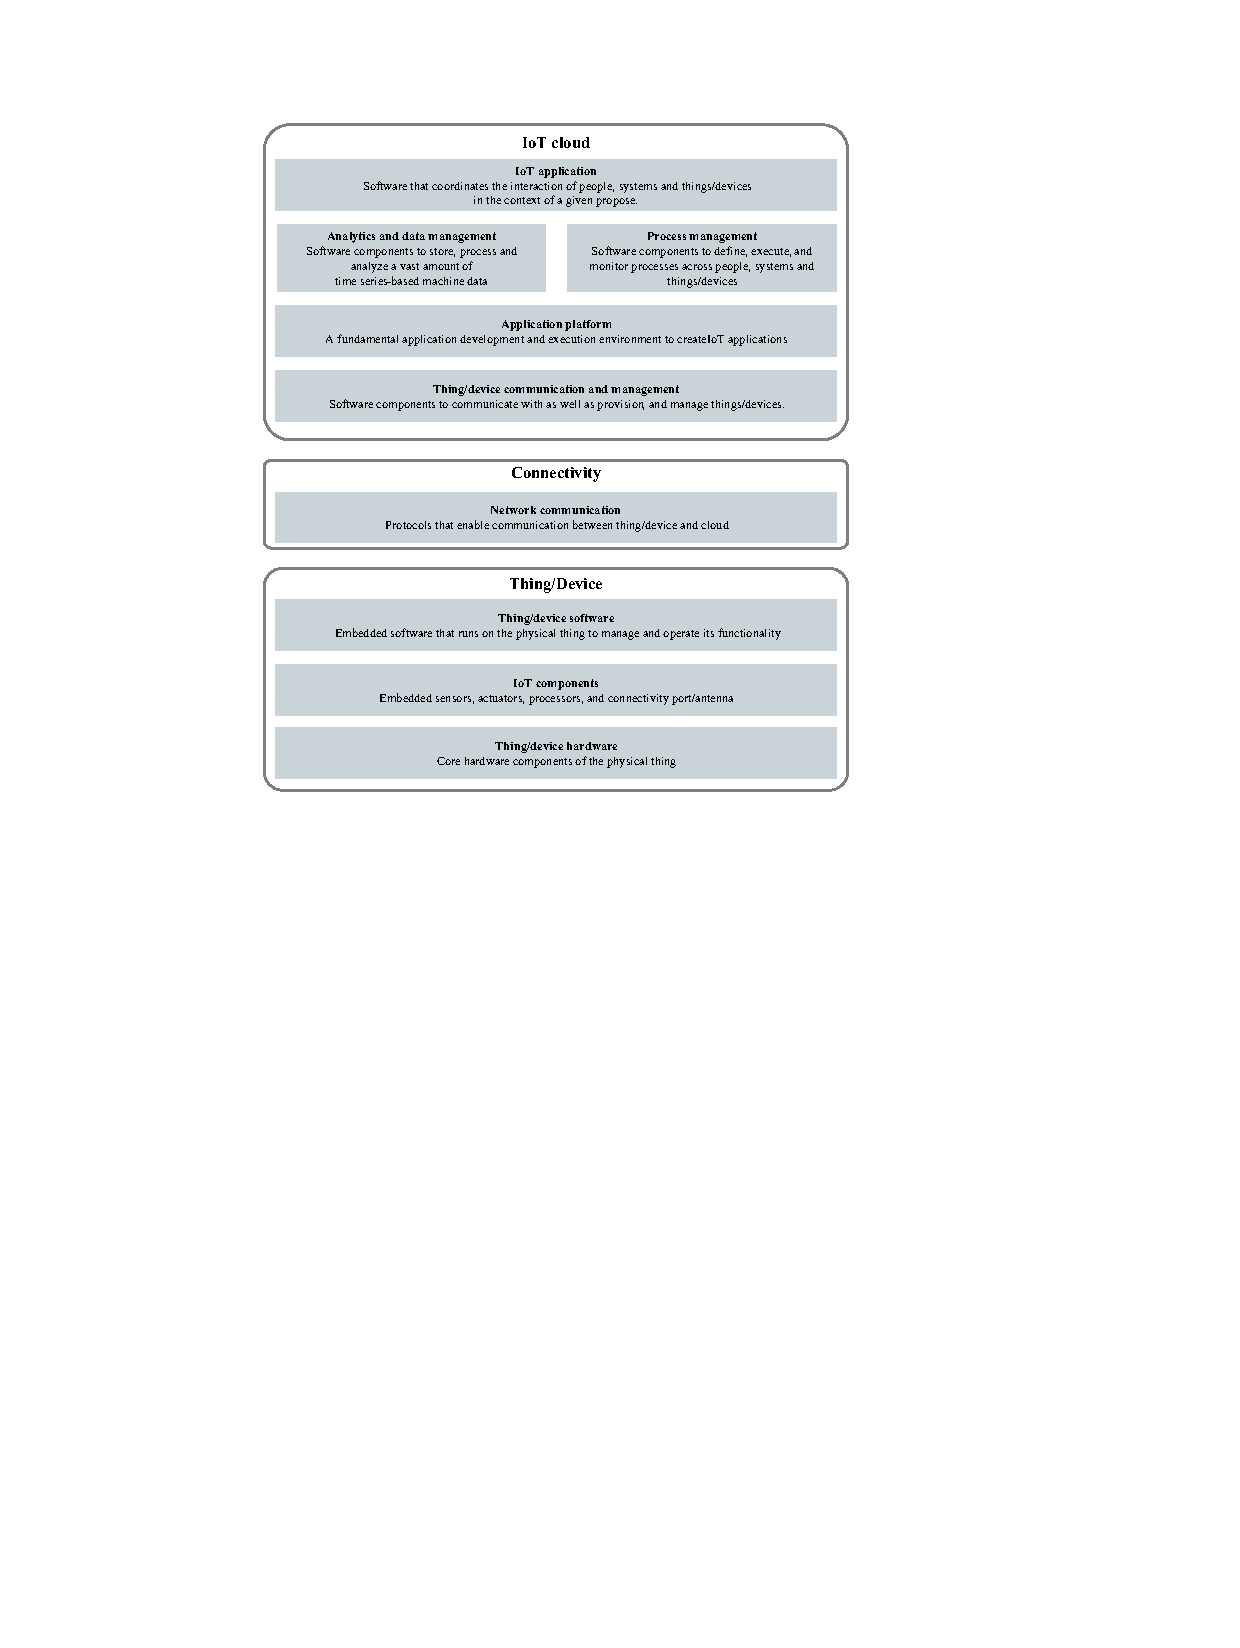
\includegraphics[scale=0.66]{Talk11/wortmann_stack.png}
	    \end{center}
	    \caption{`Internet of Things' technology stack based on Wortmann et al. \cite{wortmann}}
	    \label{fig:wortmann_stack}
    \end{figure}
	
	As a basis serves a `thing layer' which is a hardware-based sensing layer. It has the function of identifying objects and collecting information through sensors over short-range and local networks \cite{ju}. The `network layer' the transmits real-time data. It not only connects people to `things' but also allows an information flow between `things' autonomously. The data presented by the `network layer' then can be used by companies to provide optimized and personalized services which make up the top layer \cite{ju}. This `application layer' is described by Ju et al. as a ``combination of data processing and intelligence analysis to meet the industry needs to realize an intellectualized industry'' \cite[p. 883]{ju} and allows companies to achieve ``different types of intelligent application solutions'' as well as the determination of business strategies \cite[p. 884]{ju}.

	The Internet of Things has a vast potential. On one side are the customers which enjoy novel experiences through the newly connected world, whereas on the other side, there are the businesses getting involved in the IoT market with hopes of economical and reputational gains \cite{ju}. These `gains' on the business side, or better, the way to generate economical `gain' in the `Internet of Things' and how they have changed compared to value creation in traditional businesses, are the focus of the following sections.

	\subsection{Current State of IoT}
		In this section, we highlight some of the relevant findings from the Cisco IoT ecosystem study \cite{cisco}. The following three topics are of special interest, namely players, market and standardization in regard to the current state of IoT.

		The following four categories of players have been identified by Cisco \cite{cisco}: 

		\begin{enumerate}
			\item Commercial players in the offline world are mainly manufacturers producing smart appliances such as smart phones, wearables or home automation devices but also smart automobiles etc.

			\item Commercial players in the online world are companies that provide IoT-enabling services. Example companies are Amazon (Amazon Web Services), Google (Google Cloud Platform) and Microsoft (Microsoft Azure) which all offer platforms and services that target the IoT market.

			\item Research and academia will further incite the growth of IoT by creating new theories, products and materials. New innovations stem from these players that disrupt the market.

			\item Governments and utilities are the last group of players. They are the driving force for creating smart cities, smart grids and other smart infrastructure initiatives. They are the decision makers when it comes to regulation and policies for IoT technology and also play a key role in funding IoT developments.
		\end{enumerate}
		 			
		\newpage
		 			
		There are numerous markets for IoT. Besides a market for consumer goods such as smart phones, smart homes and other smart appliances, there are many more markets where IoT has a promising future:

		\begin{enumerate}
			\item \textbf{eHealth} includes such things as virtual health care, bioelectronics sensors such as heart monitoring implant, real time monitoring of vital signs and fitness monitoring. 

			\item \textbf{Transportation} ranges from smart public and private transport to other smart transportation systems such as services such as Uber and Lyft or other car-pooling appliances. 

			\item \textbf{Energy distribution} is expected to become more efficient and more resilient on supply and demand side through automation of the energy grid (smart grid).

			\item \textbf{Smart cities} are based on the idea that with the use of information and communications technology (ICT) network infrastructures are created to improve efficiency as well as development of all areas of urban life including social, business and cultural services.

			\item \textbf{Manufacturing and distribution/logistics} are being transformed due to the current trend of IoT. `Industry 4.0' or the so called `fourth industrial revolution' refer to the automation and data exchange based on cyber-physical systems and cloud computing creating a so called smart factory.

			\item \textbf{Public safety} includes, for example, early-warning system in smart cities can help preventing and mitigating catastrophes, or road-traffic safety measures and emergency medical services.

			\item \textbf{Agriculture} includes natural-resource management with GPS mapping technologies and sensors for analyzing crop yields, monitoring growth, measuring nutrient needs and many more. 

			\item \textbf{Big data analytics} help to process the vast amount of data collected by all those sensors and smart devices. Properly analyzed, this data can deliver great insights for their respective applications. This is why big data analytics will immensely benefit from IoT but contribute to its development as well.
		\end{enumerate}
		
		On the topic of standardization, Cisco found that current IoT-specific standardization activities are confined to single scopes of application e.g. health care or agriculture. Those so called `verticals' ``[...]represent islands of disjointed and often redundant development'' \cite[p.~18]{cisco}. Such a fragmentation is detrimental to the IoT market. Overcoming and preventing such fragmentations poses the challenge of standardization. There are some major standard bodies active in IoT such as the Institute of Electrical and Electronics Engineers (IEEE) or the World Wide Web Consortium (W3C). But not all of them have global reach. For businesses, application standards will enable interoperability between products. This is needed for businesses that are part of an ecosystem and rely on interoperability. Furthermore, standardization improves flexibility and prevents IoT businesses from becoming locked in in proprietary industry standards. This flexibility increases competition between companies which will in the end be beneficial for the end user and society as it leads to better products at lower prices.
	

\section{Business Model Frameworks}
\label{sec:bmf}	
	\subsection{Definitions} 
		A successful business needs to offer products or services that there is a demand for and thus can be sold to make a profit. In short, a business has to create value. A company needs to have a strategy, a way of conducting business on an operational level that will result in long term financial success, else a business is not viable and will disappear from the market sooner or later.
		A business model can be seen as a logical abstraction describing how the business operates to make a profit. A business models hence is a core factor in deciding whether your business will be driven out of market or prosper.

		A \textbf{Business Model} is defined by Osterwalder et al. as ``a description of the value a company offers to one or several segments of customers and of the architecture of the firm and its network of partners for creating, marketing and delivering this value and relationship capital, to generate profitable and sustainable revenue streams'' \cite{osterwalder2005}. The concept of the business model became important in the 1990s as the Internet began to spread and went on to become a central backbone of today's global economy since then \cite{zott}. There is no commonly accepted view as to what the business models should include \cite{morris}, \cite{osterwalder2005}, \cite{schweizer}. Achtenhagen et al. \cite{achtenhagen} stated that there has been a change from `what business models are' to `what business models are for'. In various literature, there seems to exist an agreement that a business model is `the way of doing business' for a particular firm \cite{westerlund}. At the heart of each business model stands the goal of minimizing cost and maximizing revenue \cite{ju}.
 		
 		A \textbf{Business Model Framework} is a tool to help a company in the development of its business model by presenting an overview over the business model components described above \cite{dijkman}. Two well known business model frameworks are described below. In Section~\ref{sec:mt} the `Magic Triangle' from Gassmann et al. \cite{gassmann55} is presented followed by Subsection~\ref{sec:bmc} which illustrates the business model canvas from Alexander Osterwalder \cite{osterwalder}.

	\subsection{Magic Triangle}
	\label{sec:mt}
		A successful business needs to offer products or services that there is a demand for and thus can be sold to make a profit. In short, a business has to create value. A company needs to have a strategy, a way of conducting business on an operational level that will result in long term financial success, else a business is not viable and will disappear from the market sooner or later. A business model can be seen as a logical abstraction describing how the business operates to make a profit. A business models hence is a core factor in deciding whether your business will be driven out of market or whether it prospers. Having a suitable business model is therefore essential. In fact, ``[...] business model innovators have been found to be more profitable by an average of 6\% compared to pure product or process innovators'' \cite[p.~90]{gassmann55}. With the spread of IoT, new business models need to be developed to adapt to those technological changes in the environment and seize the opportunities that arise witch such a change. But there seems to be a problem. ``Very few managers are able to explain their company's business model ad-hoc, and even fewer can define what a business model actually is in general.'' \cite[p.~90]{gassmann55}. To keep it simple, yet sufficient, Gassmann's et al. conceptualization consists of only four central dimensions: `Who', `What', `How', `Value'. 

		The Who, What, How and Value make up the Gassmann's \textbf{Magic Triangle}. The `Who' addresses the target customer group.~The `What' refers to the product or service to those customers. What is the value offered to the customer? The `Value' explains how the business model is financially viable. How is the value generated? It includes cost and revenue structures. The `How' addresses the process and activities as well as the resources and capabilities that are required for building and distributing the value propositions.		
					
		\begin{figure}[ht]
		    \begin{center}
		    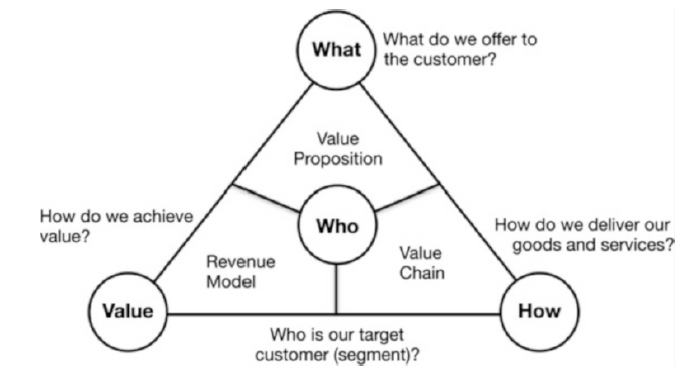
\includegraphics[scale=0.6]{Talk11/Figure1.png}
		    \end{center}
		    \caption{Gassmann's `Magic Triangle' \cite[p.~91]{gassmann55}}
		    \label{fig:m_triangle}
		\end{figure}

		The constellation of the `Magic Triangle' with the `Who' node in the middle is shown in Figure~\ref{fig:m_triangle}. Gassmann et al. argue that reducing the business model to those four components allows for a simple yet thorough enough view of the business model architecture. But creating new business models is not an easy task. It requires thinking outside the box, going beyond convention industry philosophy and can quickly become complex. Another problem is the not invented here syndrome, meaning that ideas not coming from within the company are disregarded solely because they come from the outside. As a consequence, business models should not just be copied from somewhere else but rather bring in external stimuli when generating ideas from within.

		Gassmann analyzed 250 business models in different industries from the last 25 years and as a result identified 55 pattern of business models that have served as the basis for new business models in the past. Then, together with selected companies they developed a construction methodology based on the fact that 90\% of all new business models have recombined previously existing ideas, concepts and  technologies. The BMI Navigator is the ready-to-use methodology for coming up with new business models consisting of the following three steps:

		\begin{enumerate}					
			\item Initiation: Describing the current business model is a good starting point. It creates a common ground for discussing the things that are done well and what needs improvement, and opportunities are open to be exploited. Also it get the participants started thinking in the ways of business models.

			\item Ideation: Recombining existing ideas helps generating new business models. For this purpose, Gassmann et al. condensed the 55 business models into a set of pattern cards as shown in Figure~\ref{fig:pattern_card}. Each card has a title, a description and an example. The goal is applying different cards to the current model to see what would change in this situation. The cards should trigger discussions and act as a stimuli for new innovative ideas. Open-minded team members are essential, preferably from different functions. This allows different viewpoint and thinking outside the box as well as overcoming the prevailing industry logic.
			
			\item Integration: The last step is the integration. It is obvious that a newly generated idea cannot be implemented instantaneously. New ideas need to be gradually fleshed out into fully operational business models. Considering the new stakeholders, partners and consequences for the market is crucial.
		\end{enumerate}

		\begin{figure}[ht]
		    \begin{center}
			    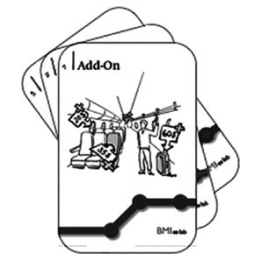
\includegraphics[scale=0.6]{Talk11/Figure2.png}
		    \end{center}
		    \caption{Pattern Card \cite[p.~95]{gassmann55}}
		    \label{fig:pattern_card}
		\end{figure}	
	\subsection{Business Model Canvas} 
	\label{sec:bmc}
		The Business Model Canvas is a strategic management tool that was developed by Alexander Osterwalder in his doctoral thesis in 2004 and later published in book form by him, Yves Pigneur and Alan Smith. \cite{osterwalder}. The tool supports business developers in gaining an overview about the key factors of their business. There are nine key factors explained by Osterwalder in detail and they are called `building blocks'. All of the building block can be aligned next to each other in a way that visualizes the mechanics of the business models (i.e. the interactions between the building block) and makes it easier to understand and discuss. The analog, pen and paper nature of the business model canvas allows it to be filled out in a team in order to stimulate creativity while finding a suitable business model for the business idea at hand.

		The usual order of filling out the business model canvas \cite[video]{bmc} is by starting with the targeted \textbf{Customer Segments}, then following with the \textbf{Value Proposition} to these customers and the \textbf{Channels} that allow the business to deliver the described value to the customer. The value is not only delivered in a physical way but there is always an emotional \textbf{Customer Relationship} with the customer involved that needs to be considered. In exchange for the proposed value, customers are willing to pay money which make up the \textbf{Revenue Streams} of the business model. With this fifth building block, the money-generating revenue side of the business model canvas is complete.

		As a counterpart for the revenue to the revenue side, every business model also includes a cost side. In Osterwalder's canvas, the cost side consists of the following four building blocks: The \textbf{Key Resources} are human, financial, physical and intellectual resources that are critical to deliver the proposed value. But resources alone do not create value - they need to be used for \textbf{Key Activities} in order for the business model to be viable. As a business owner, the decision of what part of the value you create yourself and what you let other companies do for you is written down in the \textbf{Key Partners} building block. The costs induced by resources, activities and partners are finally collected in the \textbf{Cost Structure} building block. All of these blocks are combined into one rectangular canvas as seen in Figure~\ref{fig:bmc}.

		\begin{figure}[ht]
		    \begin{center}
			    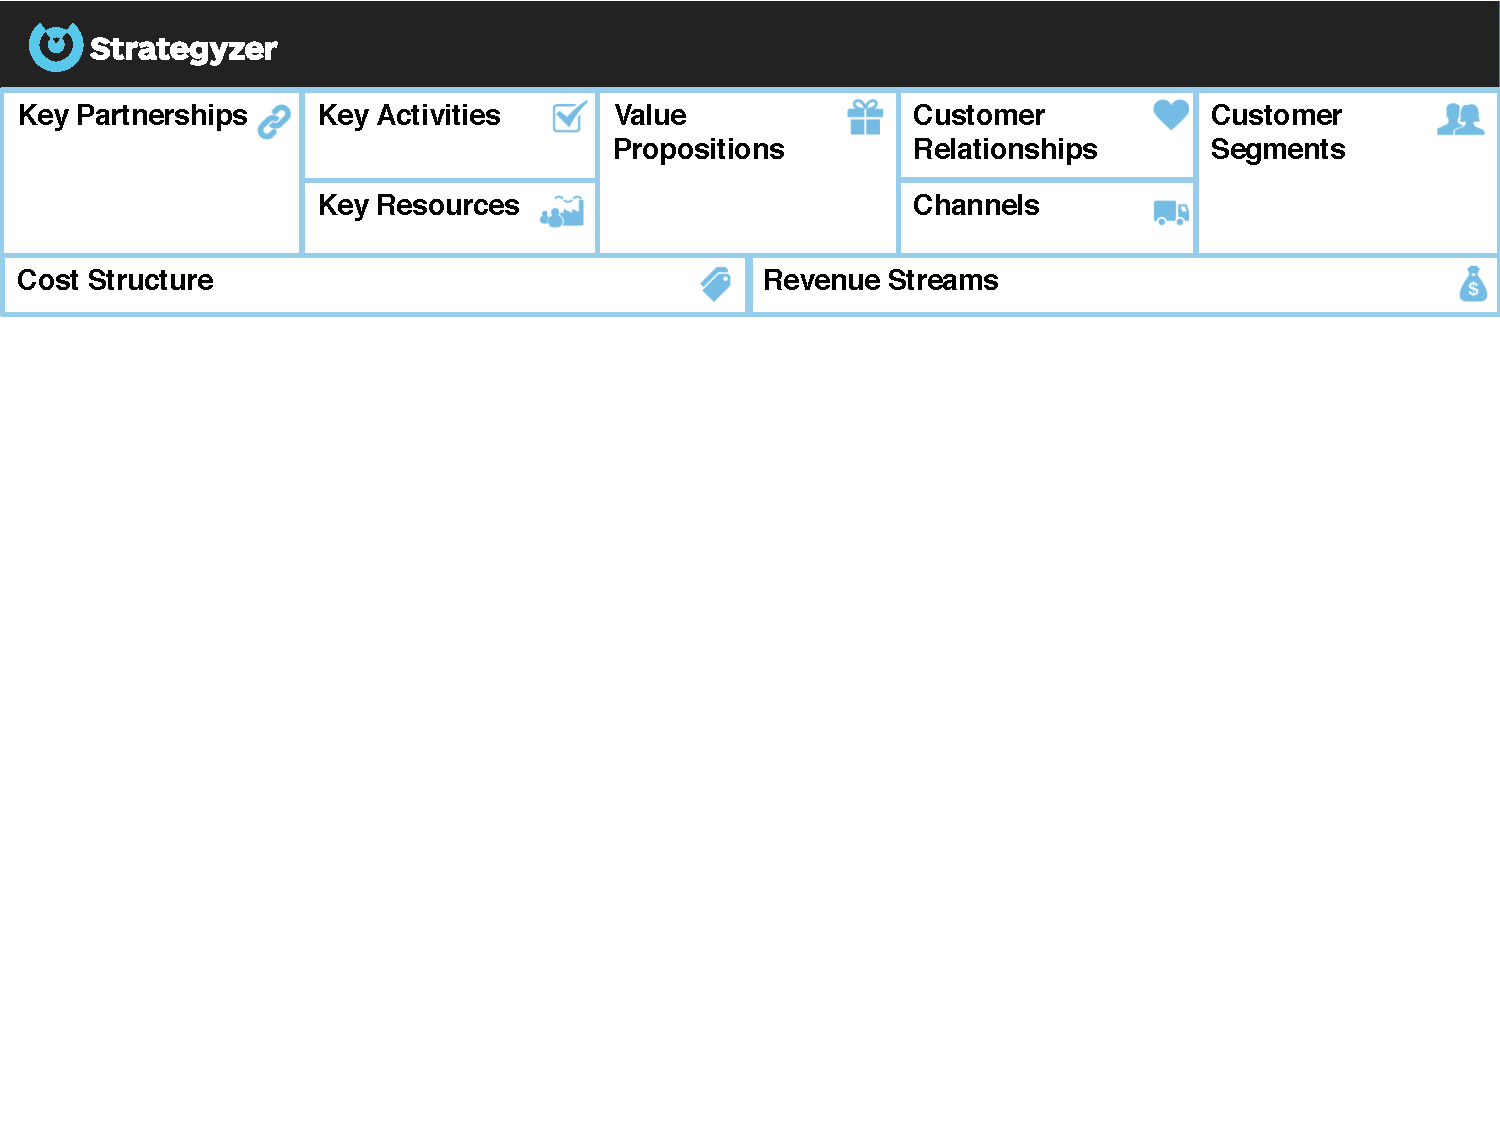
\includegraphics[scale=0.4]{Talk11/bmc_blocks_only.pdf}
		    \end{center}
		    \caption{`Business Model Canvas' (own illustration, based on Osterwalder et al. \cite{osterwalder})}
		    \label{fig:bmc}
		\end{figure}

		Each building block can be filled with different characteristics or types that are explained in detail by Osterwalder et al. in their book \cite{osterwalder}. This gives credit to the idea that new business models are mostly  recombinations of existing building blocks from other proven business models. The following paragraph will shortly summarize the options for each building block. A `Customer Segment' can be a mass market, a niche market or a multi-sided platform. Business can have very diversified customer segments, with clear or unclear segmentation. It can be important to focus on the most important customers first and align the business model primarily for them. `Value Propositions' can have various characteristics such as the newness, performance, cost reduction potential or accessibility of the proposed value. The key questions to answer with this block is `What value do we deliver to the customer?' and `Which customer needs are we satisfying?'. There can be multiple different value propositions per company. A company usually offers multiple `Channels' to serve their customers. Different customer segments may require different channels to get the product or service that the company offers. Also, the channel may differ along the different channel phases from Awareness, Evaluation, Purchase, Delivery to After sales. `Customer Relationships` differ strongly from company to company. Some forms of business models rely heavily on a personal customer relationship (e.g. barbershop) whereas for other companies, the customers might not even be known because they serve themselves in a self-service manner. `Revenue Streams` can stem from different sources and pricing models. A company can generate income through asset sale, fees for the usage, subscription, brokerage and licensing, or through advertising. Pricing models can be fixed per feature, customer segment or volume, or dynamic which means that every customer receives a different price depending on the current context. `Key Activities' include all actions that are required to offer the `Value Propositions', to run the different `Channels` and maintain the `Customer Relationships'. `Key Resources' include the physical, intellectual, human and financial assets of the company. The company pools these resources in order to turn them in an added value that can then be proposed to customers. The decision to include `Key Partners' into a company's business model can have various reasons. It might be that the partner can provide a needed component of the business model which is cheaper, which includes less risk and uncertainty for the company or which can not be provided by the company itself. The `Cost Structure' can be characterized along an axis from Cost-driven (lowest costs in the market) to Value-driven (best product/service in the market). Important characterizations of the cost structure include fixed and variable costs as well as the influence of economies of scale (the more you sell, the lower the cost per item) and economies of scope (the more diverse your offering, the more efficient a company can use its resources).

		The use of the `Business Model Canvas' as a framework to develop and explain business models is widespread in literature and practice today.
		%\todo{some source would be nice}.

\section{Available IoT Business Model Frameworks}
\label{sec:bmf_available}
	In this chapter, we will present and discuss different IoT Business Model Frameworks that are currently available in research papers. The first Subsection~\ref{subsec:fleisch} differs from the other subsections as it presents two business model patterns from Fleisch et al. that can be found in IoT business models rather than a classical business model framework. Afterwards, three different business model frameworks from Dijkman et al., Westerlund et al. and Chan are introduced. Dijkman et al. suggest a framework based on the `Business Model Canvas' discussed in Section~\ref{sec:bmc}. Westerlund et al. focuses more on the business ecosystems from a higher abstracted view and Chan presents a three dimensional collaborator model.

	\subsection{IoT Business Model Patterns}
	\label{subsec:fleisch}
		Two specific business model patterns applied in the IoT environment are described by Fleisch et al. (2014) \cite{fleisch}. This white paper is a good starting point to find out what areas a relevant IoT business model framework has to cover. The analysis of 55 distinct business model patterns from Gassmann et al. \cite{gassmann55} yields two novel business model patterns that can be applied to a IoT business ideas: `Digitally Charged Products' and `Sensor as a Service'.

		The pattern of \textbf{`Digitally Charged Products'} is described as ``classic physical products are charged with a bundle of new sensor-based digital services and positioned with new value propositions'' \cite[p.~10]{fleisch}. The components that can be used and combined are the following:

		\begin{itemize}
			\item Physical Freemium: physical asset with free digital service, premium charged service offered.
			\item Digital Add-on: cheap physical asset, digital services can be bought or activated at a high margin.
			\item Digital lock-in: limit compatibility, high dependency, unable to use another service without high switching costs.
			\item Product as Point of Sales: physical products become  sites of digital sales and marketing services.
			\item Object Self-Service: `things' can place orders autonomously over the Internet. 
			\item Remote Usage and Condition Monitoring: smart things collect and send data in real time which enables real time monitoring and error prevention.
		\end{itemize}

		This business model pattern with its six components embodies ``idea that the Internet of Things in its applications links digital services to physical products to create a hybrid bundle that is a single whole'' \cite[p.~11]{fleisch}. 

		The second pattern presented in the white paper is named \textbf{`Sensor as a Service'}. It is based around the business idea of ``collecting, processing and selling for a fee the sensor data from one subsection to other subsections'' \cite[p.~11]{fleisch}. The data gathered by the sensors itself is moved into the central focus, instead of the sensor or product itself as in the pattern `Digitally Charged Products' described above. Instead of collecting the data for one application only, it can be sold in a multi-sided market to many different stakeholders.

		As pointed out in the introduction to Section~\ref{sec:bmf_available}, Fleisch et al. do not deliver a business model framework but only two business model patterns ready to be applied to IoT business ideas.

	\subsection{Adapted Business Model Canvas for IoT}
		Dijkman et al. (2015) \cite{dijkman} analyzed current research literature in order to create a business model framework for IoT applications. They searched for papers that contained the phrasing `Internet of Things' together with `business model. Of the resulting 20 papers, only the five papers that contained actual business models were selected. Two of the five papers were based on the `Business Model Canvas' described in Section~\ref{sec:bmc}. They then identified the building blocks and building block types of business models through the selected papers and interviews with professionals working in the IoT industry. Lastly, they determined the relative importance of each building block or type through a survey. The result of Dijkman et al.'s research can be seen in Figure~\ref{fig:bm_dijkman}. The building blocks observed were equal to the building blocks from the `Business Model Canvas' described in Section~\ref{sec:bmc}. In order to `fill' the building blocks, the building block types presented by Osterwalder et al. in 2010 were merged based on the interviews, divided into multiple types, removed or extended by additional types \cite{osterwalder2010} \cite{dijkman}. The modified types are indicated in Figure~\ref{fig:bm_dijkman} using a gray colored background.

		\begin{figure}[ht]
			\begin{center}
		    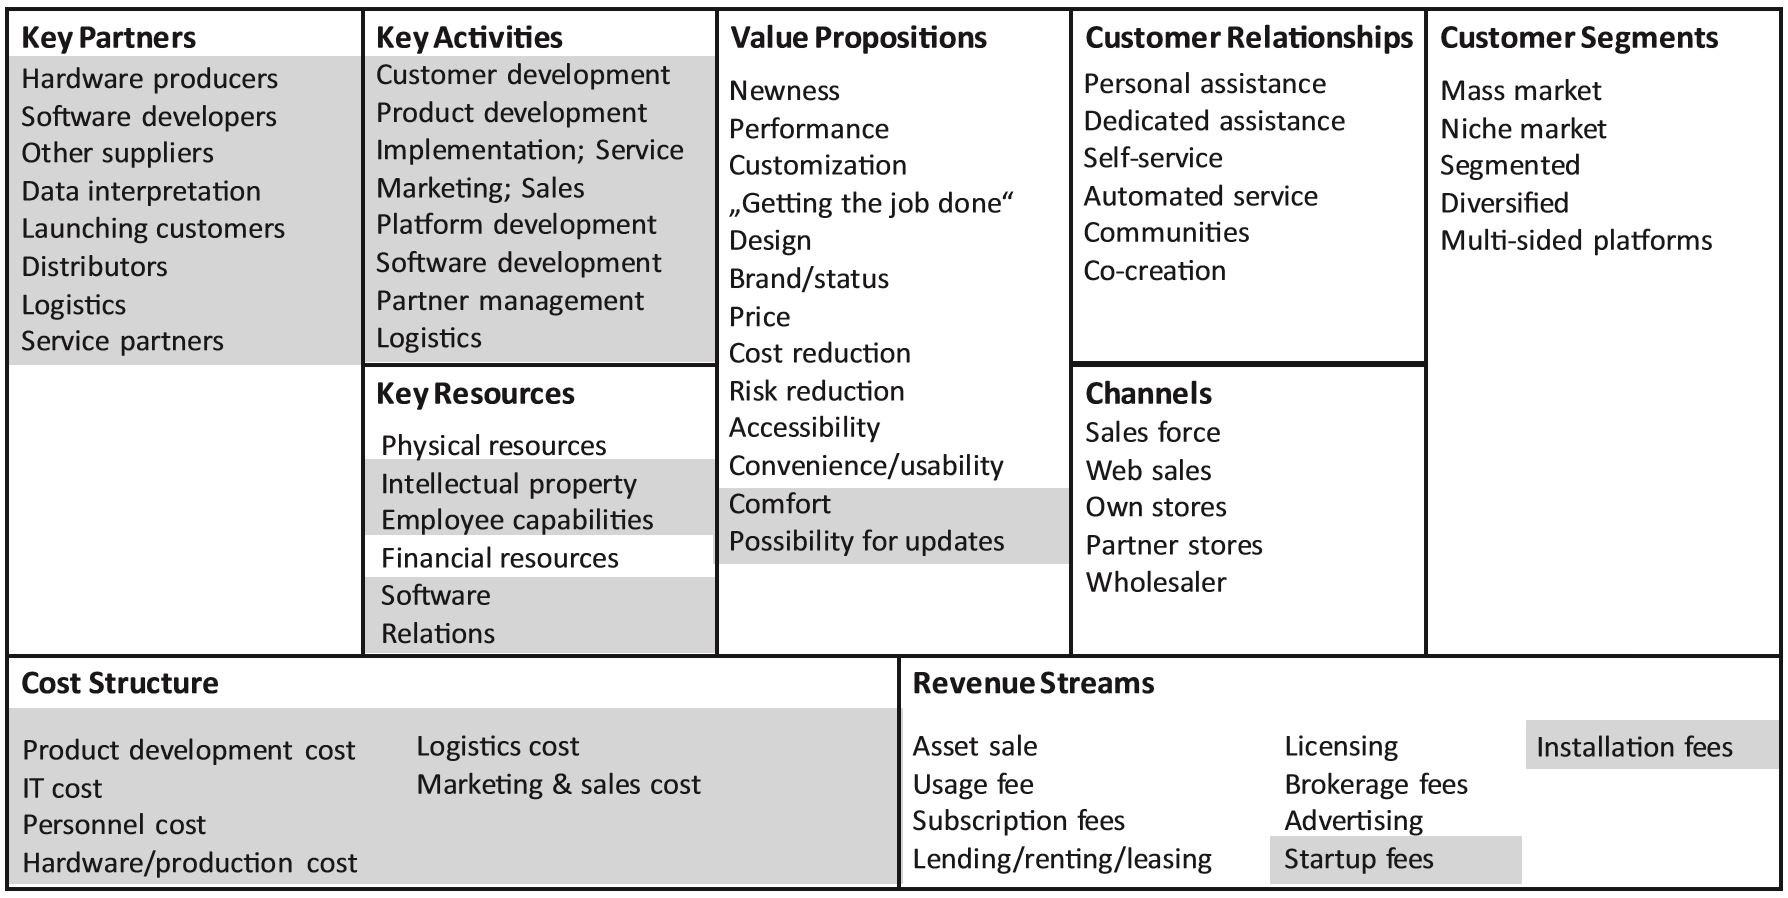
\includegraphics[scale=0.52]{Talk11/iot_canvas_dijkman.jpg}
		    \end{center}
		    \caption{Business model framework for IoT applications based on Dijkman et al. \cite{dijkman}}
		    \label{fig:bm_dijkman}
		\end{figure}

		Based on the interviews and a survey, the relative importance of each building block was determined. Dijkman et al.'s work showed, that `Value Propositions' is the most important building block in IoT business models. Furthermore, `Customer Relationship' and `Key Partners' were also considered to be more important by the interviewees. All other blocks had comparable importance results, with `channels' being slightly less important. The framework presented by Dijkman et al. can be seen as an extended classical `Business Model Canvas' \cite{bmc}. Dijkman et al. take the `Business Model Canvas' and fill it with building block types commonly used for IoT business models. Thereby, they help the user of the framework by delivering main `pillars' in the creation of a business model. These pillars can be seen as key parameters to lead the creation process into the right direction. 

	\subsection{Ecosystem Business Model Framework}
		Westerlund et al. (2014) \cite{westerlund} move from seeing IoT mainly as a technology platform to viewing it as a business ecosystem. Thus, a shift from the traditional business model of a firm to designing ecosystem business models is postulated. Such an ecosystem business model is composed of value pillars, creating and capturing value. They identified three major challenges for designing ecosystem business models namely the diversity of objects, the immaturity of innovation in the field of IoT and the unstructured nature of ecosystems in general.

		As businesses move from centralized toward decentralized and distributed network structures, they become part of complex business ecosystems. A business ecosystem can be seen an organization of economic actors. Those actors' business activities are anchored around a platform. It is argued that such systems are more than the sum of its parts and hence ``operations of the system cannot be understood by studying its parts detached from the entity'' \cite[p.~6]{westerlund}.

		Existing business model frameworks such as the `Magic Triangle' and the `Business Model Canvas' described earlier are arguably not adequate enough when it comes to analyzing such ecosystems. With the emergence of IoT, the interdependency of actors in an ecosystem gains importance due to the networks inherent to such ecosystems.

		As for all business, making money is essential. Three problems were identified  when it comes to making money in the Internet of Things:

		\begin{enumerate}
			\item `Diversity of objects' refers to the variety of different types of connected objects. Without a widespread standardization, it will be difficult to be efficient in an ecosystem. Managers will face a difficulty when trying to bring the objects, businesses and consumers together. Things can integrate with other things, requiring specific business logics.

			\item `Immaturity of innovation' refers to the current multitude of emerging technologies and components as well as innovations that have not yet matured into products and services. For IoT to be successful, modularized objects of `plug and play' nature are needed.

			\item With `unstructured ecosystems', the problem of lacking governance and underlying structures is pointed out. Unstructured ecosystems may lack essential participants for example IoT operator or potential customers. New business opportunities arise when new relationships in new industries are built or when already existing connections are extended.
		\end{enumerate}

		The ecosystem business model framework establishes a basis for building new business models to overcome these previously discussed problems and fit the ecosystem nature of IoT. The proposed framework consists of four key pillars, namely `value drivers', `value nodes', `value exchanges' and `value extract' as shown in Figure~\ref{Westerlund pillars}:

			\begin{figure}[ht]
			    \begin{center}
			    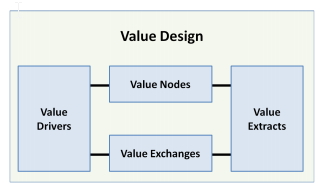
\includegraphics[scale=1.0]{Talk11/westerlundpillars.png}
			    \end{center}
			    \caption{The four pillars by Westerlund et al. \cite[p.~11]{westerlund}}
			    \label{Westerlund pillars}
			\end{figure}

		There are different \textbf{value drivers} in an ecosystem. Those value drivers are composed of both individual and shared motivation of the participants in the ecosystems. The shared motivations i.e. the shared value drivers are crucial for creating a win-win situation in a trustworthy ecosystem. Without a long-term relationship between the actors built on mutual respect of their business goals, the ecosystem will fail. Each value driver also serves as an individual value node's motivational factor. Examples of shared value drivers are cyber security and improved customer experience.

		\textbf{Value nodes} consist of various actors, activities and processes linked with other nodes to create value. Further, these nodes also can have`things' as actors. Here, smart things come into play. These self-acting `things' may be sensors, smart machines or other intelligence. Value nodes are heterogeneous as they can be organizations, networks of organizations or even network of networks.

		\textbf{Value Exchanges} take place between but also within different value nodes in the system. The value exchanged can be resources, knowledge and information. Thus, the value can be both tangible as well an intangible. Value exchanges are best described as a flow that powers `the engine'. Value exchanges are important because they describe how revenues are generated and distributed in the ecosystem.

		As not all created value is meaningful in regard to commercialization, only specific parts of created value make sense to extract. \textbf{Value extract} refers to the part of the ecosystem that extracts value. That means it focuses on what can be monetized and what the relevant nodes and exchanges for the value creating and capture are. The concept of value extract is useful to gain focused view on what is actually relevant in the ecosystem for monetization. Each business in the ecosystem needs to have something that is beneficial for them from the business point of view. Value extract can be single activities, automated processes, individuals, commercial organizations, non-profits or even groups of organizations or networks with their respective value flows between their nodes.

		Westerlund et al.'s business model framework heavily focuses on the value part of business models. Based on the concept of value design, those four value pillar described above come together in a single picture. Value design is an architecture mapping the foundational structure of the ecosystem business model. It provides boundaries for an ecosystem and gives a pattern of operation.

	\subsection{Three-dimensional Collaborator Model Framework}
		The three-dimensional collaborator model presented by Chan (2015) \cite{chan} builds on a model described by Holler et al. \cite{holler}. The three dimensions of Chan's model are `Who', `Where' and `Why'. On first sight, those dimensions seem similar to the nodes in Gassmann et al.'s `Magic Triangle' proposition but the differences become evident once the meaning behind the three dimensions is investigated. The `Who' describes the collaborating partners that build the value network. The `Where' refers to sources of value co-creation and lastly the `Why' describes how partners actually benefit from collaborating within the value network \cite{chan}. Figure~\ref{fig:chan} shows the table of the proposed framework. While those three dimensions are not explicitly visible, the individual components in the framework address them indirectly.

		\begin{figure}[ht]
		    \begin{center}
		    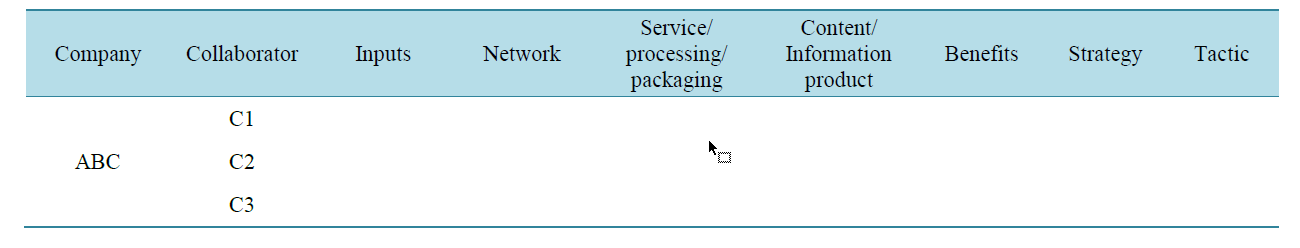
\includegraphics[scale=0.5]{Talk11/chan.png}
		    \end{center}
		    \caption{Chan's business model framework \cite[p.~559]{chan}}
		    \label{fig:chan}
		\end{figure}

		Chan applied his framework on multiple case studies to explore the `Who', `Where' and `Why' elements of his business model framework. A closer look at one example of the Hong Kong Communications Co., Ltd (HKC) company helps to understand how the framework applied to a use case. The Wong Tai Sin Temple in Hong Kong is a popular tourist attraction. With over 5 million visitors per year, the information board at the temple containing detailed information about the temple's history becomes inaccessible to many visitor during peak seasons. Due to the lack of a communication system, the management was unable to estimate the visitor count and to allocate the required manpower. With the help of a real time location tracking system and a mobile application, visitors now have access to self-serving tour guide services. The free mobile application allows customers to access introductory videos and information at each attraction point without the assistance of tourist guides \cite[p.~560]{chan}. 

		\begin{figure}[ht]
		    \begin{center}
		    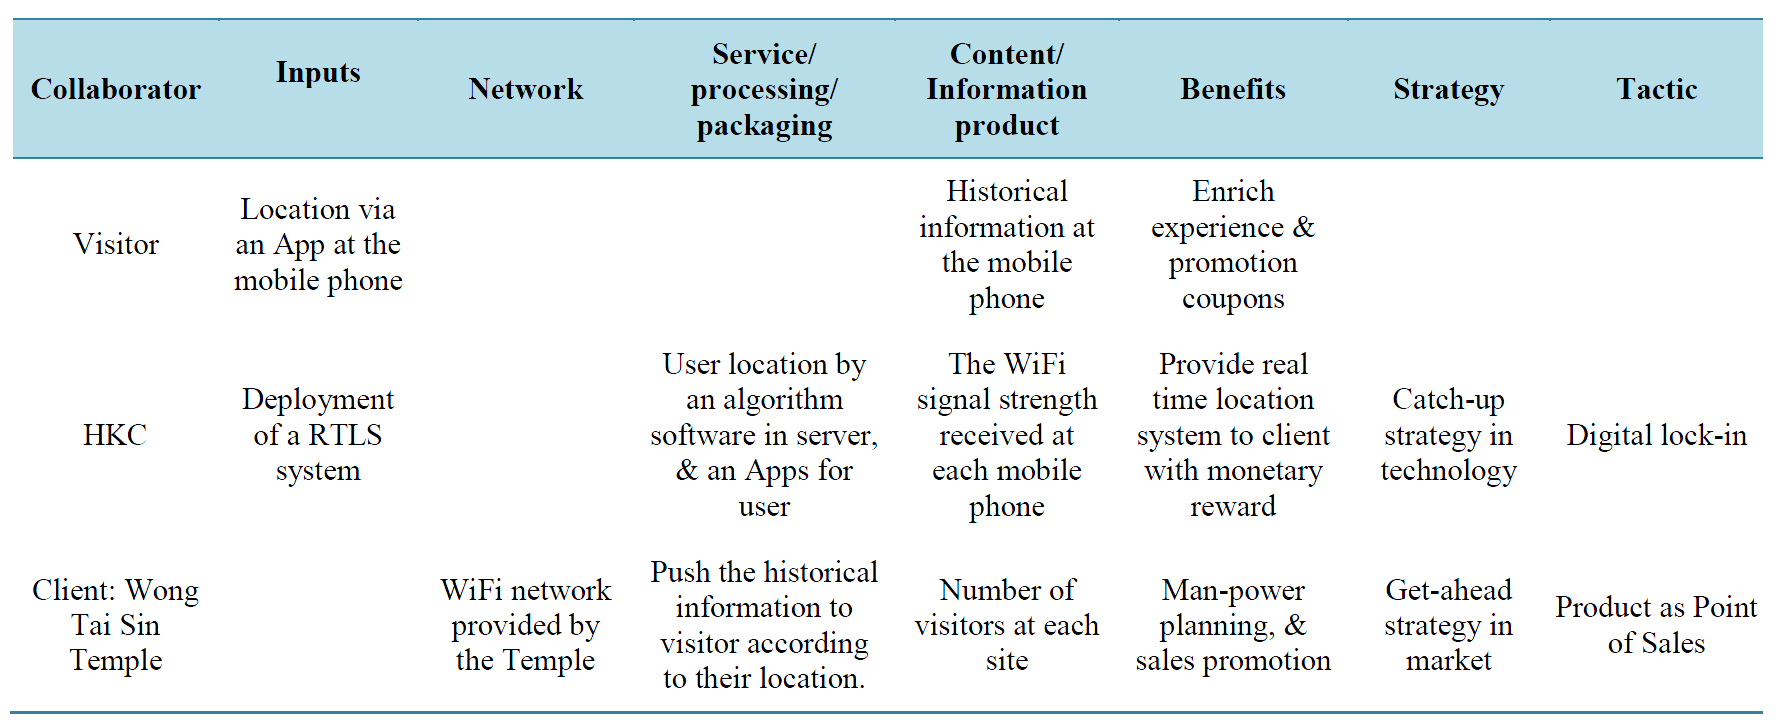
\includegraphics[scale=0.4]{Talk11/chanexample.png}
		    \end{center}
		    \caption{Chan's business model framework applied to the HKC use case \cite[p.~560]{chan}}
		    \label{fig:chan_ex}
		\end{figure}

		Figure \ref{fig:chan_ex} shows the according business model. Interesting are the columns `Strategy' and `Tactic'. Li et al.,(2012) \cite{li} proposed four IoT strategy categories which are adapted by Chan in the use cases for his three-dimensional business model framework. The strategies are `get-ahead strategy in market', `catch-up strategy in market', `get-ahead strategy in technology', and `catch-up strategy in technology'. Get-ahead strategies enable the firm to stay ahead of other competitors, giving them a first mover advantage. Catch-up strategies, on the other hand, are intended to follow and learn from the industrial leaders by operational efficiency and quality \cite{chan}.
		Besides strategy, the business model framework contains the `Tactic' column. The six components of the `Digitally Charged Products' pattern by Fleisch et al. \cite{fleisch} as presented in Subsection~\ref{subsec:fleisch} are the proposed tactics to choose from.

\section{Comparison of available IoT Business Model Frameworks using a case study}
\label{sec:bmf_comparison}
	In the following section, we will introduce a fictitious company in order to make it possible to compare the available business model frameworks and illustrate their respective strengths and weaknesses.

	\subsection{Introduction to the Case Study Company}
		Our case study company is called `FlexSpace'. It offers an integrated beacon and software solution for companies to make the usage of companies' office space more flexible by showing the available desk places in an office building to employees. This allows the customer companies to use office buildings more efficiently and thereby reduce the square meters per employee which directly saves money for the company. A beacon is a miniature, battery-powered radio transmitter that usually employs  Bluetooth Low Energy (BLE) technology to communicate with nearby devices. These beacons allow letting the employees check-in at their desk using their smartphones. `FlexSpace' offer the installation and maintenance of the described beacon infrastructure at customer sites as well as a white-label mobile application for their customers. The application displays the available desk places and enables the user to check-in at a specific desk using the closest beacon available. The visual appearance can be customized per customer to fit the customer company's corporate design.

	%\subsection{IoT Business Model Patterns (Fleisch et. al, 2014)}

	\subsection{Adapted Business Model Canvas for IoT}
		Based on the IoT adapted `Business Model Canvas' Framework by Dijkman et al., a business model for `FlexSpace' was created. The Business Model Framework presented in Figure~\ref{fig:bm_dijkman} was filed out and customized for the needs of `FlexSpace'. The resulting Business Model can be seen in Figure~\ref{fig:bmc_flex}.
			\begin{figure}[ht]
			    \begin{center}
			    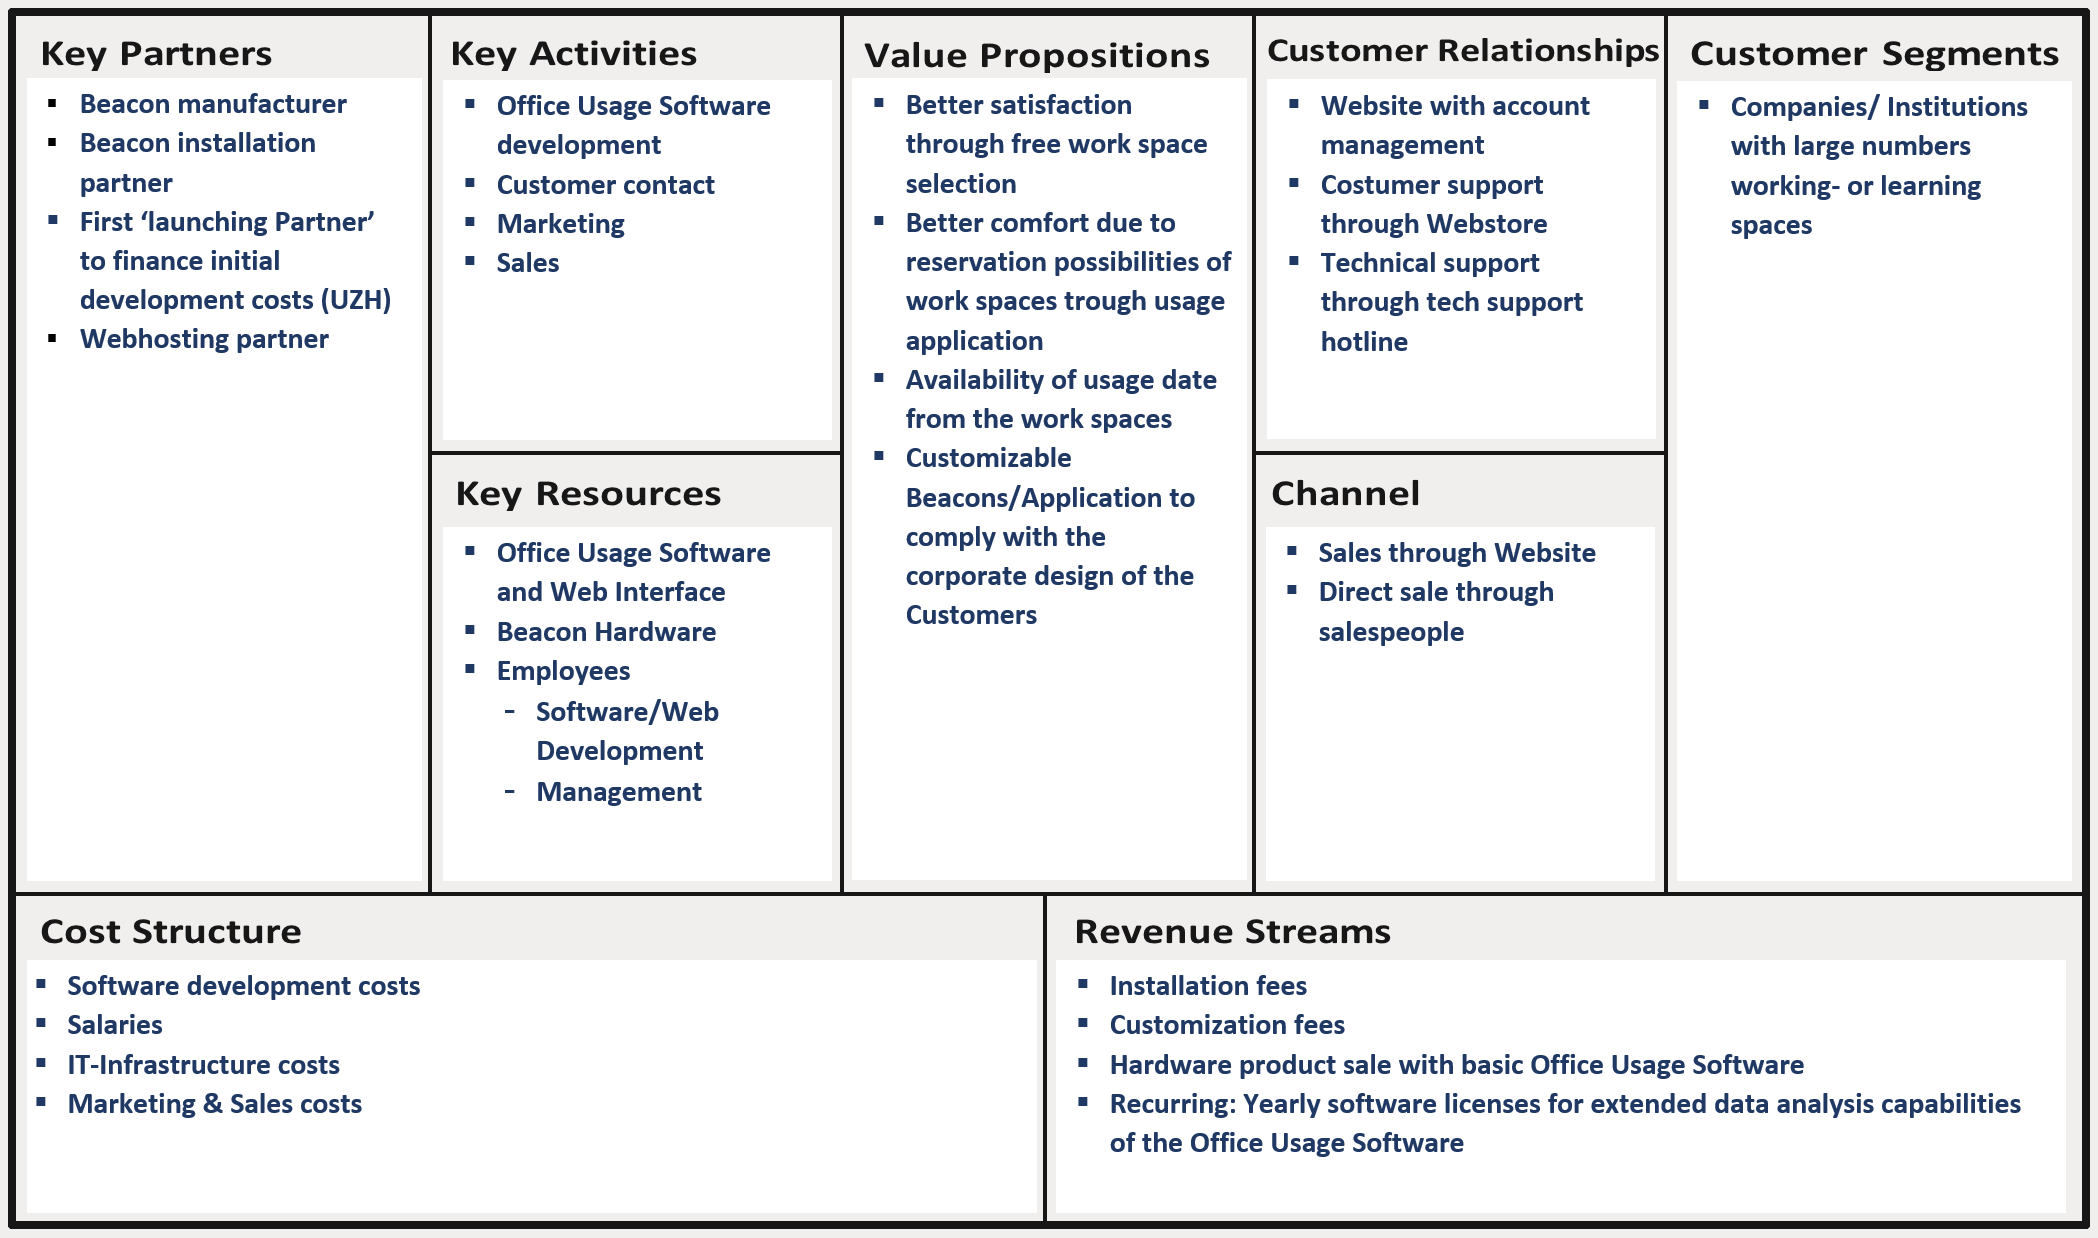
\includegraphics[scale=0.50]{Talk11/bmc_flex.png}
			    \end{center}
			    \caption{Dijkman's Business Model Canvas Framework applied for the FlexSpace company (own illustration based on \cite{dijkman} and \cite{bmc})}
			    \label{fig:bmc_flex}
			\end{figure}
		The `Key Partners' block contains the producers of the beacon hardware. For this building block, it is crucial to have a `launching partner'. This needs to be a big customer that finances the initial development. A suitable partner would be the University of Zurich (UZH) as it has many learning spaces that could be managed using the beacon-based approach. Other partners are the beacon installation partner as well as a web hosting provider for the corporate website enabling account management. The `Key Activities' are software development as well as traditional activities such as marketing, sales or customer contact. The `Key Resources' needed are mainly employees with respective skill sets, the beacon hardware and the corresponding software. In the `Cost Structure' block, the relevant costs for running the `FlexSpace' business are listed. The important ones are development costs, salaries and marketing and sales. Dijkman et al. \cite{dijkman} rated `Value Proposition' as the most important building block of a business model. For `FlexSpace', the following value proposition were found important:

		\begin{itemize}
			\item The overview over all working spaces allows more convenient searching for free work places.
			\item Due to remote reservation possibilities, a higher comfort can be achieved. 
			\item The available usage space data allows the analysis of work space usage for further optimizations.
			\item The customers of `FlexSpace' are able to customize the beacons and the software to achieve high compliance with their corporate design.  
		\end{itemize}  

		The `Customer Relationships' are maintained through the website as well as through a technical support hotline. The `Channel' block describes how the customers will be reached. The primary channels are through the website and through sales persons directly approaching customers. The important customers in `Customer Segments' are companies or institutions with large numbers of working spaces. The revenue generation in the building block `Revenue Streams' contains installation and customization fees of the beacons. The biggest revenue is generated through one-time sales of the beacons with the corresponding configuration software and recurring revenue through yearly licenses for the full Office Usage software including web-services and data analysis capabilities. It can be seen that a big part of the proposed framework from Dijkman et al. was used in the generation of the business model. Some proposed components were excluded e.g. due to the chosen distribution channels (no partner stores). The resulting business model promises to be specific enough to be useful for the creation of the `FlexSpace' business. 

	\subsection{Ecosystem Business Model Framework}
		Westerlund et al. suggest ``that managers need to shift their focus from `the business model' of a firm" to `ecosystem business models''' \cite[p.~8]{westerlund}. The application of the framework proposed by them leads us to the following business model for FlexSpace:

		\begin{enumerate}
			\item Value Drivers: Sustainability (less office space per employee), increased employee satisfaction (employee can choose his own desk place) and availability of usage data

			\item Value Nodes: FlexSpace Employee, Beacons, Beacon Manufacturer, Beacon Installation Partner, Managers, Employees, Office Usage Application (data processing), Internal IT department

			\item Value Exchanges: Beacon from manufacturer to Location from employee to beacon, data from beacon to office usage application, information from office usage application to manager, knowledge from FlexSpace Employee to Manager

			\item Value Extract: Installation Process, Software Licensing, Provision from installation partners, Training fees to learn how to use the Office Usage Application
		\end{enumerate}

	\subsection{Three-dimensional Collaborator Model Framework}
		When we apply Chan's framework to our fictional company, Figure~\ref{use case chan} shows a possible result. The emphasis on the mutual benefits for all collaborators becomes evident. Thanks to the beacons at each desk where the employees check-in, the target company now knows about the used capacity of workplaces. They can analyze which employees come on premise to work and who rather works from home. The software provided can measure changes in utilization over the year. Predictions for flexible allocations can be made to adjust the varying demand for workplaces over the year. Employees profit by being free to choose where they want to work and do not risk running into an occupied workplace again. FlexSpace's benefit is essentially the monetary reward.

		\begin{figure}[ht]
		    \begin{center}
		    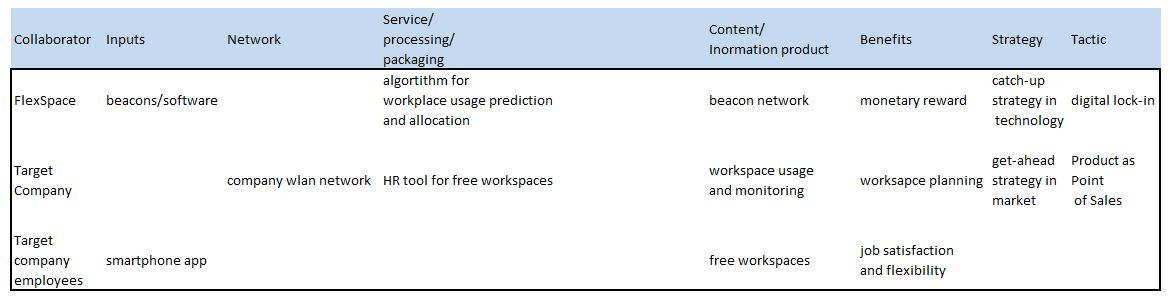
\includegraphics[scale=0.55]{Talk11/chanexampleusecase.jpg}
		    \end{center}
		    \caption{Chan's framework applied to our company}
		    \label{use case chan}
	    \end{figure}

\section{Evaluation and Discussion}
\label{sec:eval}

	\subsection{Changes in Business Models due to the Emergence of IoT}
		Business models for IoT differ from traditional business models. This subsection takes a look at what changed due to the emergence of IoT.

		Sticking to the `Business Model Canvas', Dijkman et al. \cite{dijkman} do not provide a new framework per se, but rather show relative importance of the individual building blocks for IoT businesses. Unsurprisingly, the `Value Propositions' building block has by far the highest relative importance compared to the other block. Generally speaking, an emphasis on value creation and capture as well as an emphasis on a more networked environment can be observed. Hui \cite{hui} states that in industries that are becoming connected, differentiation, cost, and focus are no longer mutually exclusive. Rather than that, they can be mutually reinforcing in creating and capturing value.

		In the ecosystem business model framework by Westerlund et al. \cite{westerlund}, there is a dogmatic shift. The business model is no longer seen on the level of a single company like traditional business models do. Rather, the concept of value design is applied on an ecosystem level. Such a conception of business models in an ecosystem may be more suitable considering the nature of IoT. Networking, interconnections, interconnectivity and thus interdependence come with the territory when talking about IoT. IoT in itself is an ecosystem that can be scaled from only personal devices such as wearables to huge networks such as smart cities. In smart cities, there are many actors and stakeholders. Identifying ecosystems within a smart city and thus finding shared and private value drivers allow businesses to cooperate efficiently with each other in a win-win environment. Traditional business models lack an ecosystem view. With ecosystem business model frameworks, an important and aspect inherent to IoT can be addressed and monetized on that other traditional business models fail to reach. Naturally such a business model becomes more complex and skilled managers are needed for a successful implementation. The focus on the firm level needs to be extended to a broader view. Connections to new industries have to be made which is not an easy task, but is needed for businesses to break into the emergent IoT market and prove themselves and offer their customer value. Nevertheless, this ecosystem business model framework also shares some similarities with traditional business model frameworks. In its core, value design is a concept found in many business models. As can be seen in the `Magic Triangle' by Gassmann \cite{gassmann55}, `Value' is one of the nodes that make up the `Magic Triangle' and is thus essential for the business model to work. Furthermore the pillars in the ecosystem business model framework can be categorized, compared and examined in the same way that the vertices in the `Magic Triangle' or building blocks of the `Business Model Canvas' can.

		However, the ecosystem business model framework may be too abstract to be yet applied to businesses as we can see in our use case. Chan himself states that they simply provided grounds for a novel tool for designing ecosystem business models which has to be further studied and developed. In contrast, Chan's three dimensional collaborator framework proves its usefulness in the use cases. Similar to the ecosystem business model, it focuses on the multitude of actors who benefit from each other. Besides the emphasis on collaborators, concrete benefits for all participants are captured in the model and the new components `Strategy' and `Tactic' enrich the model. Chan's business model framework is specifically tailored for the needs of IoT companies.	
	
	\subsection{Case Study Evaluation}
		The business model framework from Dijkman et al. \cite{dijkman} is a template based on the `Business Model Canvas' \cite{bmc}. It contains the important building block types that should be considered in the creation of an IoT business model. The template is easy to use and easily adaptable to custom needs whilst reminding to the networking perspective of IoT. The business model creation process does not depend on Dijkman's et al. framework, it could also be done using the classical `Business Model Canvas' albeit requiring more care to not unintentionally omit IoT specific business model parts.
		With regards to the applied `FlexSpace' example, it can be said that the application was rather simple, the predefined business model parts of the framework reduced the complexity of the business model generation greatly.

		Applying Westerlund et al.'s framework leads to the following observations: First, FlexSpace is not a typical ecosystem business idea. A typical example of a ecosystem business would be a multi-sided platform such as the Apple AppStore. This might be the reason why the application of the framework was difficult. Also, the authors themselves stated that their paper only proposes the four key value pillars that can be used as a basis for the development of a practically applicable business model framework tool in the future. The application of Westerlund et al.'s framework showed clearly that more work is needed to turn this ``plum pudding model'' \cite[p. 10]{westerlund} into a practical tool for business model creation.

		Chan's model proved itself already in many case studies in the original paper. Unsurprisingly, it also works really well for our case study and proved to be less abstract than the ecosystem framework by Westerlund et al.. It provides us with a comprehensive view from how collaborator benefit from each other to what strategies and tactics are used. Same as the business model canvas from Dijkman et al., it provides an easy and ready-to-use template to fill out. By taking the ecosystem aspect into account, we find that in Westerlund's framework a clear differentiation from Dijkman is visible whose framework does not address this aspect. \todo{Why reference to Westerlund..?} \cite{westerlund}.

		Whatever approach businesses will choose in the future, the most important thing is to realize that IoT brings in perspectives which are not explicitly addressed by traditional business model frameworks. Thus one is well advised to take action early and keep an open mind when it comes to business models for IoT. Some business may be better off sticking to the well-known `Business Model Canvas' while other may profit by a adapting an ecosystem business model view. What businesses should definitely avoid is to fall for the well-known `boiling frog syndrome' by not acting until it is too late. As long as there are still profits coming in, why take a risk and leave your comfort zone? Competition and environmental factors are always in movement. What works today may not work anymore in a few years. The `boiling frog syndrome' states that gradually increasing problems go unnoticed or are not dealt with until it is too late to tackle them. A frog in a pot of water will not jump out of the water when it is slowly brought to boil. When the water gets too hot for him, his muscles are too weak to jump out. Likewise, a business that has diminishing returns year after year may not be concerned about the little loss between consecutive years. When they realize the devastating loss suffered over multiple years, there are no resources left to tackle the problem and they go bankrupt. That's why ignoring the changes IoT brings with itself may lead to a devastating result for companies unwilling to adapt.

\section{Summary and Conclusion}
\label{sec:summary}

	This paper starts by presenting the essentials of the `Internet of Things' paradigm and the concept of business models in general. After building a common ground, the classic business model frameworks were introduced. Based on literature research, the currently important business model frameworks for IoT businesses were then presented and described. The illustrated frameworks were compared based on an imaginary model company. A general comparison of the frameworks revealed that there exists a shift from the classical single firm-based business model view to a more ecosystem-based structure of business models for the `Internet of Things'. The application of the presented frameworks to the model company revealed that Dijkman's et al. framework provided the most complete and simple experience to create a new business model. Chan's collaborator framework was also ready to use although it required more attention to get the `complete picture' of the business model. Positively stood out, the ecosystem based-view on the constructed business model weighted the characteristics network-oriented business models more than Dijkman et al. Westerlund et al.'s value pillars framework was hard to apply to the model company. It focuses on the value-oriented part of business models and seemed overly abstract for a day-to-day usage scenario. 

	The literature on business models for IoT is relatively scarce, thus this paper is based on few self referencing papers e.g. \cite{ju} and \cite{dijkman} and lacks a broader view which reflects in this paper. Future research containing a large-scale field study could strengthen the current IoT business model frameworks, and help some frameworks to adapt and mature into a framework usable for real-world use cases.

	To conclude, the only more generally usable framework is the adapted business model canvas from Dijkman et al.. This framework finds the balances between the originally empty business model canvas and a completely predefined IoT business model solution. A deeper analysis of each block could lead to a more specific framework which would then in turn only be usable for a subsection of businesses.

 \begin{thebibliography}{99}
	\bibitem {achtenhagen} L. Achtenhagen, L. Melin, L. Naldi: \emph{Dynamics of Business Models - Strategizing, Critical Capabilities and Activities for Sustained Value Creation}, Long Range Planning, 2013, 46(6): 427-442. \url{http://dx.doi.org/10.1016/j.lrp.2013.04.002},  last visit: November 17, 2016.
 
 	\bibitem {echo} Amazon Echo, \url{https://www.amazon.com/dp/B00X4WHP5E}, last visit: November 17, 2016.

	\bibitem {atzori} L. Atzori, A. Iera, G. Morabito: \emph{The internet of things: a survey}, Computer Networks 54:2787-2805, 2010 

	\bibitem {chan} H.C.Y. Chan: \emph{Internet of Things Business Models}, Journal of Service Science and Management, 8, 552-568. \url{http://dx.doi.org/10.4236/jssm.2015.84056}, last visit: November 17, 2016.

	\bibitem {cisco} CISCO: \emph{IEEE-SA Internet of Things Ecosystem Study}, IEEE Standards Association, New York, 2015, \url{http://www.cisco.com/c/dam/en/us/solutions/collateral/industry-solutions/dlfe-670918525.pdf}, last visit: November 17, 2016.

	\bibitem {cho} M.-H. Cho: \emph{South Korea to invest \$5b by 2020 in IoT and smart cars}, 2015, \url{http://www.zdnet.com/article/south-korea-to-invest-5b-by-2020-in-iot-and-smart-cars/}, last visit: November 17, 2016.

	\bibitem {dijkman} R.M. Dijkman, B. Sprenkels, T.Peeters, and A. Janssen: \emph{Business Models for the Internet of Things}, International Journal of Information Management, Vol 35, pp 672-678, 2015.

	\bibitem {fleisch} E. Fleisch, M. Winberger, F. Wortmann: \emph{Business Models and the Internet of Things}, Bosch Internet of Things \& Services Lab, pp 1-19, August 2014, \url{http://www.iot-lab.ch/?page_id=10543}, last visit: November 17, 2016.

 	\bibitem {gartner} Gartner: \emph{4.9 Billion Connected ``Things'' Will Be in Use in 2015}, 2014, \url{http://www.gartner.com/newsroom/id/2905717}, last visit: November 17, 2016.
	
	\bibitem {gassmann} O. Gassmann, K. Frankenberger, and M. Csik: \emph{Revolutionizing the business model.} in O. Gassmann and F. Schweitzer (Eds.), Management of the Fuzzy Front End of Innovation. Springer, New York, pp. 89-97, 2014, \url{http://link.springer.com/chapter/10.1007%2F978-3-319-01056-4_7}, last visit: November 17, 2016.

	\bibitem {gassmann55} Gassmann et al.: \emph{Geschaeftsmodelle entwickeln: 55 innovative Konzepte mit dem St. Galler Business Model Navigator.} in Hanser Verlag, 2013.

	\bibitem {holler} J. Holler, V. Tsiatsis, C. Mulligan, S. Avesand, S. Karnouskos, D. Boyle: \emph{From Machine-to-Machine to the Internet of Things: Introduction to a New Age of Intelligence}, Elsevier, Waltham.
	
	\bibitem {hui} G. Hui: \emph{How the Internet of Things Changes Business Models}, Harvard Business Review, July 24, 2014, \url{https://hbr.org/2014/07/how-the-internet-of-things-changes-business-models}, last visit: November 17, 2016.

 	\bibitem {ifttt} IFTTT, \url{https://ifttt.com/}, last visit: November 17, 2016.

 	\bibitem {itu} ITU: \emph{New ITU standards define the internet of things and provide the blueprints for its development}, \url{http://www.itu.int/ITU-T/newslog/New+ITU+Standards+Define+The+Internet+Of+Things+And+Provide+The+Blueprints+For+Its+Development.aspx}, last visit: November 17, 2016.

 	\bibitem {ju} Jaehyeon Ju, Mi-Seon Kim and Jae-Hyeon Ahn: \emph{Prototyping Business Models for IoT Service}, Procedia Computer Science, 91, pp. 882 - 890, 2016, \url{http://www.sciencedirect.com/science/article/pii/S1877050916312911}, last visit: November 17, 2016.
 	
 	\bibitem {kickstart} Kickstarter, \url{https://www.kickstarter.com/}, last visit: November 17, 2016.

	\bibitem {li} Y. Li, M.J. Hou, H. Liu, Y. Liu: \emph{Towards a Theoretical Framework of Strategic Decision, Supporting Capability and Information Sharing under the Context of Internet of Things}, Information Technology and Management, 13, 205-216, 2012, \url{http://dx.doi.org/10.1007/s10799-012-0121-1}, last visit: November 17, 2016.

  	\bibitem {lifx} \url{http://www.lifx.com/}

	\bibitem {miller} B. Miller: \emph{Obama Places \$160 Million Bet on Smart Cities, Internet of Things}, 2015, \url{http://www.govtech.com/Obama-Places-160-Million-Bet-on-Smart-Cities-Internet-of-Things.html}, last visit: November 17, 2016.

	\bibitem {morris} M. Morris, M. Schindehutte, J. Allen: \emph{The Entrepreneur's Business Model: Toward a Unified Perspective}, Journal of Business Research, 58: 726-35. \url{http://dx.doi.org/10.1016/j.jbusres.2003.11.001}, last visit: November 17, 2016.

	\bibitem {osterwalder2005} A. Osterwalder, Y. Pigneur, C. L. Tucci: \emph{Clarifying Business Models: Origins, Present and Future of the Concept}, Communications of the Association for Information Science, 16(1): 1-25, 2015, \url{http://aisel.aisnet.org/cais/vol16/iss1/1}, last visit: November 17, 2016.

	\bibitem {osterwalder} A. Osterwalder, Y. Pigneur, A. Smith: \emph{Business Model Generation}, self published, 2010.


	\bibitem {osterwalder2010} A. Osterwalder, Y. Pigneur:  \emph{Business model generation: a handbook for visionaries, game changers, and challengers}, 2010, Hoboken, NJ: John Wiley \& Sons

 	\bibitem {port_hepp} M.E. Porter, J.E. Heppelmann: \emph{How smart, connected products are transforming competition}, Harvard Business Review 92:11-64
	
	\bibitem {rossi} B. Rossi: \emph{How the Internet of Things is Changing Business Models}, Information Age - Insight and analysis for IOT leaders, May 4, 2016 \url{http://www.information-age.com/it-management/strategy-and-innovation/123461371/how-internet-things-changes-business-models}, last visit: November 17, 2016.

	\bibitem {schweizer} L. Schweizer: \emph{Concept and Evolution of Business Models. Journal of General Management},  31(2): 37-56.

	\bibitem {bmc} Strategyzer AG: \emph{The Business Model Canvas}, \url{https://strategyzer.com/canvas/business-model-canvas}, last visit: November 17, 2016.

 	\bibitem {tilley_nest}  A. Tilley: \emph{Google Acquires Smart Thermostat Maker Nest For \$3.2 Billion. 2014}, \url{http://www.forbes.com/sites/aarontilley/2014/01/13/google-acquires-nest-for-3-2-billion/#7049b3181416}, last visit: November 17, 2016.

 	\bibitem {tilley_smart}  A. Tilley: \emph{Samsung Acquires SmartThings, A Fast-Growing Home Automation Startup}, 2014, \url{http://www.forbes.com/sites/aarontilley/2014/08/14/samsung-smartthings-acquisition-2/#25b90c197965}, last visit: November 17, 2016.

	\bibitem {westerlund} M. Westerlund, S. Leminen and M. Rajahonka: \emph{Designing Business Models for the Internet of Things} Technology Innovation Management Review, July 2014, \url{http://timreview.ca/article/807}, last visit: November 17, 2016.

	\bibitem {wortmann} F. Wortmann and K. Fluechter: \emph{Internet of things. Business \& Information Systems Engineering}, 2015. 57(3): p. 221-224.

	\bibitem {zott} C. Zott, R. Amit, and L. Massa, \emph{The business model: recent developments and future research}, Journal of management, 2011. 37(4): p. 1019-1042. 
 \end{thebibliography}

